\documentclass[12pt]{article} %lineno

\usepackage[top=0.8in,left=1.2in, right=1.2in, bottom=1in]{geometry}
\usepackage{graphicx}
\usepackage{hyperref}
\usepackage{multirow}
\usepackage{caption}
\usepackage{listing}

\usepackage{pgf}

\usepackage{alltt}

\hypersetup{colorlinks=true, linkcolor=blue, filecolor=blue, urlcolor=blue,
citecolor=blue }

\renewcommand{\figurename}{\textbf{Figure}}
\renewcommand{\thefigure}{\textbf{S\arabic{figure}}}

\renewcommand{\tablename}{\textbf{Table}}
\renewcommand{\thetable}{\textbf{S\arabic{table}}}

\renewcommand{\baselinestretch}{1.3}

\begin{document}


\title{Supplementary Material for ``LinguaPhylo: a probabilistic model specification language for reproducible phylogenetic analyses''}

\date{}

\author{
Alexei J. Drummond\textsuperscript{1,2,3}*,
Kylie Chen\textsuperscript{1,2,3},
F\'{a}bio K. Mendes\textsuperscript{1,4},
Dong Xie\textsuperscript{1,2,3}
}

\maketitle 

{\small
\noindent \textbf{1} Centre for Computational Evolution, University of Auckland, Auckland, New Zealand
\\
\textbf{2} School of Biological Sciences, University of Auckland, Auckland, New Zealand
\\
\textbf{3} School of Computer Science, University of Auckland, Auckland, New Zealand
\\
\textbf{4} Department of Biology, Washington University in St. Louis, St. Louis, United States\\
}

\medskip

\noindent *Corresponding author: a.drummond@auckland.ac.nz

\clearpage

% \section{Example LPhy script}

\subsection*{RSVA example}
% An accompanying tutorial for this analysis is publicly available at \url{www.linguaphylo.gihub.io/tutorials/time-stamped-data/}.
% We have modified the script slightly for illustrative purposes:

{
  \small
  \begin{listing}
    % \stepcounter{example}
    \begin{alltt}
    data \{
      options = \{\textcolor{gray}{ageDirection=}\textcolor{magenta}{"forward"}, \textcolor{gray}{ageRegex=}\textcolor{magenta}{"s(\textbackslash{}d+)"}\};
      nexusFilePath = \textcolor{magenta}{"tutorials/data/RSV2.nex"};
      D = \textcolor{magenta!80!black}{readNexus}(\textcolor{gray}{file=}nexusFilePath, \textcolor{gray}{options=}options);
      codon = D.\textcolor{magenta!80!black}{charset}([\textcolor{magenta}{"3-629\textbackslash{}3"}, \textcolor{magenta}{"1-629\textbackslash{}3"}, \textcolor{magenta}{"2-629\textbackslash{}3"}]);
      n = 3;
      L = [209, 210, 210];
      taxa = D.\textcolor{magenta!80!black}{taxa}();
    \}
    model \{
      \textcolor{green}{\(\pi\)} ~ \textcolor{blue}{Dirichlet}(\textcolor{gray}{replicates=}n, \textcolor{gray}{conc=}[\textcolor{magenta}{2.0}, \textcolor{magenta}{2.0}, \textcolor{magenta}{2.0}, \textcolor{magenta}{2.0}]);
      \textcolor{green}{\(\kappa\)} ~ \textcolor{blue}{LogNormal}(\textcolor{gray}{sdlog=}\textcolor{magenta}{0.5}, \textcolor{gray}{meanlog=}\textcolor{magenta}{1.0}, \textcolor{gray}{replicates=}n);
      \textcolor{green}{r} ~ \textcolor{blue}{WeightedDirichlet}(\textcolor{gray}{conc=}\textcolor{magenta!80!black}{rep}(\textcolor{gray}{element=}\textcolor{magenta}{1.0}, \textcolor{gray}{times=}n), \textcolor{gray}{weights=}L);
      \textcolor{green}{\(\mu\)} ~ \textcolor{blue}{LogNormal}(\textcolor{gray}{meanlog=}\textcolor{magenta}{-5.0}, \textcolor{gray}{sdlog=}\textcolor{magenta}{1.25});
      \textcolor{green}{\(\Theta\)} ~ \textcolor{blue}{LogNormal}(\textcolor{gray}{meanlog=}\textcolor{magenta}{3.0}, \textcolor{gray}{sdlog=}\textcolor{magenta}{2.0});
      \textcolor{green}{\(\psi\)} ~ \textcolor{blue}{Coalescent}(\textcolor{gray}{taxa=}taxa, \textcolor{gray}{theta=}\textcolor{green}{\(\Theta\)});
      Q = \textcolor{magenta!80!black}{hky}(\textcolor{gray}{kappa=}\textcolor{green}{\(\kappa\)}, \textcolor{gray}{freq=}\textcolor{green}{\(\pi\)}, \textcolor{gray}{meanRate=}\textcolor{green}{r});
      \textcolor{green}{codon} ~ \textcolor{blue}{PhyloCTMC}(\textcolor{gray}{L=}L, \textcolor{gray}{Q=}Q, \textcolor{gray}{mu=}\textcolor{green}{\(\mu\)}, \textcolor{gray}{tree=}\textcolor{green}{\(\psi\)});
    \}
    \end{alltt}
    % \captionof{subexample}{LPhy script specifying a phylodynamic model
    \caption{An LPhy script for phylodynamic analysis of a virus dataset containing Respiratory syncytial virus subgroup A (RSVA) genomic samples.
    \newline}
    \label{lphy:rsva}
    \end{listing}
}
Example \ref{lphy:rsva} shows an LPhy script for performing phylogenetic inference on a virus dataset containing sequences of the Respiratory syncytial virus subgroup A (RSVA). 
This script concisely specifies a phylogenetic analysis using 19 lines of code.  
The code contains a \textbf{data block} for specifying the input dataset, and a \textbf{model block} which defines the phylogenetic model. 

% \newpage

\begin{figure}
  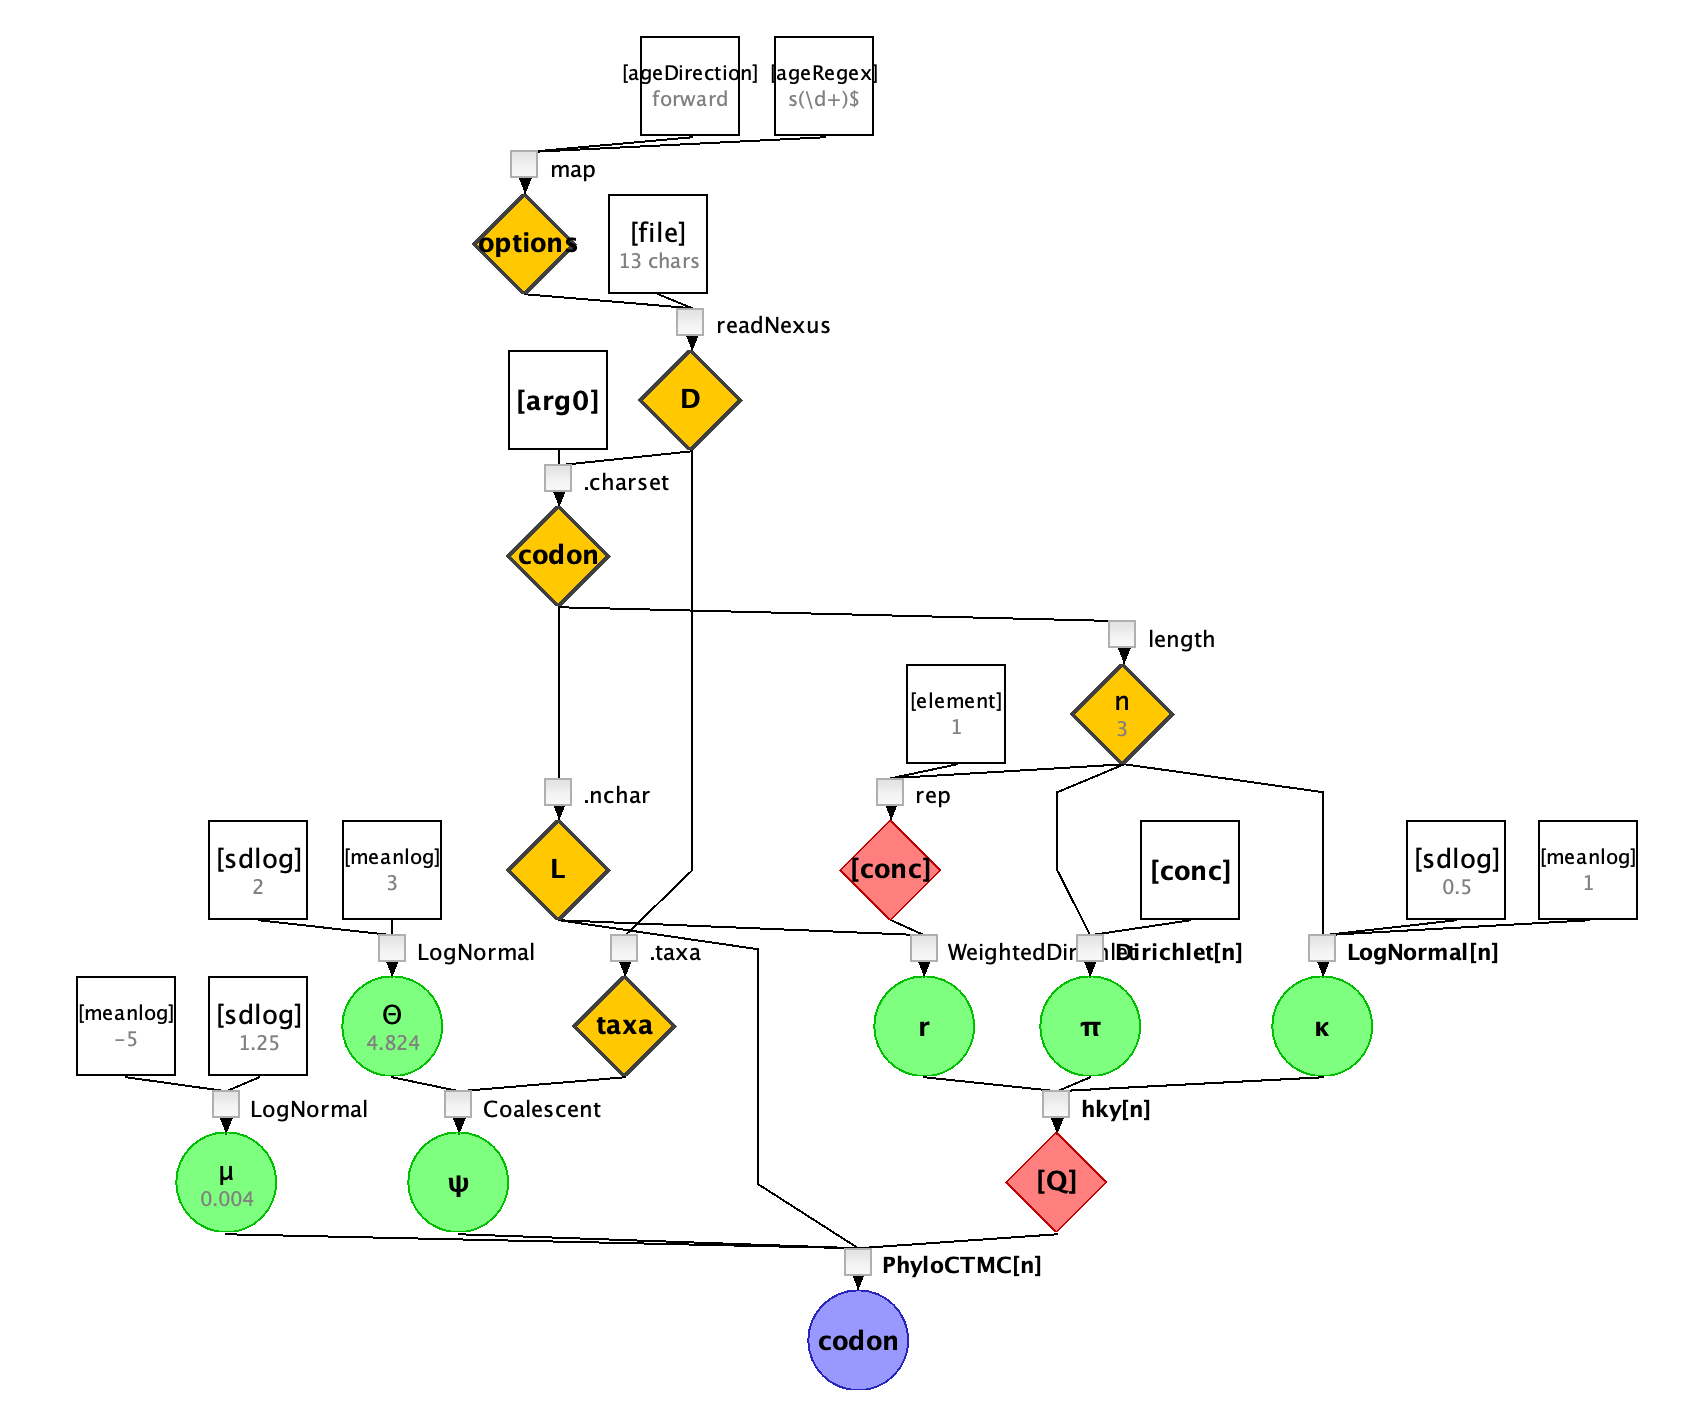
\includegraphics[width=\textwidth]{figs/RSV2.png}
  \caption{A screenshot of the probabilistic graphical model of Example \ref{lphy:rsva}.} 
  \label{fig:RSV2PGM}
\end{figure}


\clearpage


\bigskip

%\textbf{This PDF file includes:}

%\medskip 

%Figures XX to XX

%\medskip

%Tables XX to XX

% \newpage 

% \begingroup
% \pagestyle{plain}
% \listoffigures
% \listoftables
% \endgroup

% \newpage

% Figures go here



% Tables

\begin{table}
\small
\centering
\begin{tabular}{ l | l | l }
    \hline\hline
    Function & Brief & Examples \\ 
    \hline\hline
    binaryRateMatrix & binary trait rate matrix & errorModel1.lphy, errorModel2.lphy\\  
    f81 & F81 model\cite{felsenstein1981} & f81Coalescent.lphy\\  
    generalTimeReversible & general time reversible rate matrix & h5n1.lphy \\  
    gtr & GTR model\cite{tarvare1986some} & gtrCoalescent.lphy\\  
    hky & HKY model\cite{hasegawa1985dating} & hkyCoalescent.lphy\\  
    jukesCantor & Jukes-Cantor model\cite{jc69} & jcCoalescent.lphy\\  
    k80 & K80 model\cite{kimura1980simple} & \\  
    lewisMK & LewisMK model\cite{lewis2001likelihood} & lewisMKCoalescent.lphy\\  
    migrationMatrix & population process rate matrix & simpleStructuredCoalescent.lphy\\  
    wag & WAG model\cite{whelan2001general} & wagCoalescent.lphy\\  
    \hline
\end{tabular}

\label{tab:ratematrix}
\caption{LPhy functions to produce the instantaneous rate matrix.}
\end{table}

\begin{table}
\small
\begin{tabular}{ l | l | l }
    \hline\hline
    Generative distribution & Brief & Examples \\ 
    \hline\hline
    MultispeciesCoalescent & multispecies coalescent & simpleMultispeciesCoalescent.lphy, \\ & & simpleMultispeciesCoalescentTaxa.lphy, \\ & & twoGeneMultispeciesCoalescent.lphy\\  
    Coalescent & Kingman's coalescent \cite{Rodrigo1999SerialCoalescent} & RSV2.lphy \\  
    SkylineCoalescent & skyline coalescent prior\cite{drummond2005bayesiansequences} & hcv\_col.lphy\\  
    StructuredCoalescent & Structured coalescent\cite{muller2017structured} & simpleStructuredCoalescent.lphy\\  
    \hline
\end{tabular}

\label{tab:coalescent}
\caption{The coalescent tree generative distributions in LPhy.}
\end{table}

\begin{table}
\scriptsize
\begin{tabular}{ l | p{8cm} | p{4cm} }
    \hline\hline
    \bf Generative distribution & \bf Brief & \bf Examples \\ 
    \hline\hline
    BirthDeathSampling & birth-death-sampling tree\cite{stadler2011mammalian,stadler2012estimatingdata} & birthDeathRhoSampling.lphy\\  
    BirthDeathSerialSampling & birth-death serial sampling tree\cite{stadler2013dating} & simpleBirthDeathSerial.lphy\\  
    BirthDeath & calibrated birth-death\cite{heled2015calibrated} & simpleCalibratedBirthDeath.lphy, \\ & & simpleExtantBirthDeath.lphy\\  
    FossilBirthDeathTree & fossilized birth-death process\cite{heath2014fossilized} & simFossilsCompact.lphy\\  
    FullBirthDeath & birth-death tree\cite{kendall1948generalized} & simpleFullBirthDeath.lphy\\  
    RhoSampleTree & birth-death tree sampled from a larger tree & \\  
    SimBDReverse & complete birth-death tree with both extant and extinct species & simFossils.lphy\\  
    SimFBDAge & A tree of extant species and those sampled through time & simFBDAge.lphy\\  
    SimFossilsPoisson & A tree with fossils added to the given tree at rate psi & simFossils.lphy\\  
    Yule & Yule tree\cite{yule1925ii} & simpleYule.lphy, \\ 
    & & yuleRelaxed.lphy\\  
    \hline
\end{tabular}

\label{tab:coalescent}
\caption{The birth-death tree generative distributions in LPhy.}
\end{table}

\begin{table}
\scriptsize
\begin{tabular}{ l | l | l }
    \hline\hline
    Generative distribution & Brief & Examples \\ 
    \hline\hline
    PhyloBrownian & phylogenetic Brownian motion process\cite{felsenstein1973maximum} & simplePhyloOU.lphy\\  
    PhyloCTMC & phylogenetic continuous time Markov process\cite{felsenstein1981} & simpleBModelTest.lphy\\  
    PhyloMultivariateBrownian & phylogenetic multivariate Brownian motion & simplePhyloMultivariateBrownian.lphy\\  
    PhyloOU & phylogenetic Ornstein-Ulhenbeck process\cite{felsenstein1973maximum} & simplePhyloBrownian.lphy\\  
    \hline
\end{tabular}

\label{tab:coalescent}
\caption{The sampling distributions that the phylogenetic likelihood is derived from in LPhy.}
\end{table}

\begin{table}
\footnotesize
\begin{tabular}{ l | p{7cm} | l }
    \hline\hline
    Generative distribution & Brief & Examples \\ 
    \hline\hline
    Bernoulli & coin toss distribution prior & simpleRandomLocalClock.lphy, \\ & & simpleBModelTest.lphy\\  
    Beta & beta distribution prior & birthDeathRhoSampling.lphy, \\ & & simpleBModelTest.lphy\\  
    Cauchy & cauchy distribution prior & \\  
    Dirichlet & dirichlet distribution prior & birthDeathRhoSampling.lphy, \\ & & dirichlet.lphy\\  
    DiscreteUniform & discrete-uniform prior & simpleBModelTest.lphy, \\ & & simpleBModelTest2.lphy\\  
    DiscretizeGamma &  discretize-gamma prior & gtrGammaCoalescent.lphy, \\ & & simpleBModelTest.lphy\\  
    Exp & exponential distribution prior & birthDeathRhoSampling.lphy, \\ & & yuleRelaxed.lphy\\  
    ExpMarkovChain & smoothing prior\cite{drummond2005bayesiansequences} & skylineCoalescent.lphy\\  
    Gamma & gamma distribution prior & covidDPG.lphy\\  
    Geometric & geometric distribution prior & \\  
    InverseGamma & inverse-gamma  distribution prior & totalEvidence.lphy\\  
    LogNormal & log-normal distribution prior & hkyCoalescent.lphy, \\ & & errorModel1.lphy\\  
    Normal & normal distribution prior & simplePhyloBrownian.lphy, \\ & & simplePhyloOU.lphy\\  
    NormalGamma & normal-gamma distribution prior & simplePhyloBrownian.lphy, \\ & & simplePhyloOU.lphy\\  
    Poisson & poisson distribution prior & expression4.lphy, \\ & & simpleRandomLocalClock2.lphy\\  
    RandomBooleanArray & samples a random boolean array & simpleRandomLocalClock2.lphy\\  
    RandomComposition & samples a random k-tuple of positive integers that sum to n & skylineCoalescent.lphy\\  
    Uniform & uniform distribution prior & simFossilsCompact.lphy\\  
    Weibull & weibull distribution prior & \\  
    WeightedDirichlet & weighted dirichlet distribution prior & totalEvidence.lphy, \\ & & weightedDirichlet.lphy\\  
    \hline
\end{tabular}

\label{tab:prior}
\caption{The prior distributions in LPhy.}
\end{table}

\begin{table}
\begin{tabular}{ l | l | l }
    \hline\hline
    Function & Brief & Examples \\ 
    \hline\hline
    aminoAcids & amino acid data type & wagCoalescent.lphy\\  
    binaryDataType & binary data type & \\  
    nucleotides & nucleotide data type & primates2.lphy\\  
    standard & the standard data type & totalEvidence.lphy\\  
    \hline
\end{tabular}
\label{tab:coalescent}
\caption{The alignment data type in LPhy.}
\end{table}

\begin{table}
\begin{tabular}{ l | l | l }
    \hline\hline
    Function & Brief & Examples \\ 
    \hline\hline
    nucleotideModel & bModelTest\cite{bouckaert2017bmodeltestcomparison} rate matrix & simpleBModelTest.lphy, \\ & & simpleBModelTest2.lphy\\  
    bModelSet & bModelTest model set & simpleBModelTest.lphy\\  
    bSiteRates & site rates for the given bModelTest parameters & simpleBModelTest2.lphy\\  
    bSiteModel & bModelTest site model & simpleBModelTest.lphy\\  
        \hline
\end{tabular}
\label{tab:coalescent}
\caption{Bayesian phylogenetic site model averaging in LPhy.}
\end{table}

\clearpage

\bibliographystyle{plain}

\bibliography{linguaPhylo}


\end{document}